\section{The CLSAdvection concept}
The idea of CLSAdvector was inspired by Roenby \textit{et al.} who proposed isoAdvector concept\cite{isoAdvector}, which is a geometric VOF method. In the isoAdvector method, void fraction $\alpha$ is interpolated into the vertexes of the grids. Generally, it is customary to visualize the interface by showing the 0.5-isosurface based on the void fraction $\alpha$ with the post-processing procedure, like ParaView$^{\textregistered}$. However, it is not precise to use 0.5-isosurface as interface because it can hardly cut the cell into two subcells of the volumetric proportions dictated by the volume fraction $\alpha$. So the most important step of isoAdvector is to find the exact value of $\alpha$ that can cut the surface cells into two subcells with right void proportions. This method is quite novel and it is applied to unstructured meshes and implemented as an incompressible two-phase flow VOF solver in OpenFOAM$^{\textregistered}$. However, isoAdvector still has the same faults as other geometric VOF methods, in which the curvature and normal direction of interface are influenced by the discontinuous property of $\alpha$. Different from the isoAdvector method, CLSAdvector uses the projection distance D of $\vec{x}_j$ (the vector from cell center to \textit{i}-th vertex) on interface normal direction $\vec{n}$ to reconstruct the interface that meets void fraction $\alpha$. For the sake of clarity, only ideas about CLSAdvector are focused in this section, and the numerical detailed description of the implementations can be found in section 3. The reader is referred to the source code provided at this website\cite{CLSAdvector}.
\subsection{Governing equations for incompressible two phase flow}
%Navier-Stokes Momentum equation
The incompressible Navier-Stokes equations for two immiscible phases(A and B) read
\begin{equation}\label{1}
\frac{\partial \mathbf{u}}{\partial t}
+ \mathbf{u}\cdot\nabla\mathbf{u}
=
-\frac{1}{\rho}\nabla{p}
+\frac{1}{\rho}\nabla\cdot(2\mu{D})
+\mathbf{f_\Gamma}
+\mathbf{g}
\end{equation}
%Navier-Stokes Conservative equation
\begin{equation}\label{2}
\nabla\cdot\mathbf{u}=0
\end{equation}
where $\mathbf{u}$ is the velocity, $\rho$ is the density, \textit{p} is the pressure, $\mathbf{g}$ is the gravitational acceleration and $\mu$ is the dynamic viscosity. The material properties are constant for each phase and discontinuous at the interface. To avoid numerical instability \cite{son2002coupled}, it is needed to make fluids properties in a continuous form as follows
\begin{equation}\label{16}
\rho=\rho_A + (\rho_B-\rho_A)H(\phi),
\end{equation}
and
\begin{equation}\label{17}
\mu=\mu_A + (\mu_A-\mu_B)H(\phi).
\end{equation}
In equation \ref{1}, D is defined as the rate of deformation tensor,
\begin{equation}\label{3}
D=\frac{\nabla\mathbf{u}+{\nabla\mathbf{u}}^T}{2}.
\end{equation}
$\mathbf{f_\Gamma}$ is the surface tension force, which is transformed to be a volume force scattering within the interface region by CSF (continuum surface force) model\cite{brackbill1992continuum} as follows
\begin{equation}\label{4}
\mathbf{f_\Gamma}
=
\frac{\sigma\kappa\nabla{H_\varepsilon(\phi)}}{\rho_\varepsilon(\phi)}.
\end{equation}
At the interface $\Gamma$, separating the two fluids, there is the normal continuity condition for velocity
\begin{equation}\label{5}
u_{A,\perp}-u_{B,\perp}
=
\mathbf{u}_A\cdot\mathbf{n}
-
\mathbf{u}_B\cdot\mathbf{n}
\equiv
0,
\end{equation}
the tangential continuity condition for velocity
\begin{equation}\label{6}
u_{A,\parallel}-u_{B,\parallel}
\equiv
0,
\end{equation}
and the jump condition for surface stress
\begin{equation}\label{7}
  [\mathbf{n}\cdot(-p\mathbf{I}+2\mu{D})\cdot\mathbf{n}]=\sigma\kappa,
\end{equation}
where $\mathbf{I}$ is the identity matrix, $\sigma$ is the surface tension and $\kappa$ is the interface curvature. According to the article\cite{van2008computing}, if viscosity is continuous across the interface, the coupled jump condition of pressure and velocity gradient(\ref{7}) can be decoupled. Then we can get
\begin{equation}\label{14}
[\nabla\mathbf{u}]_\Gamma = 0,
\end{equation}
and
\begin{equation}\label{15}
[p]_\Gamma=\sigma\kappa.
\end{equation}
The curvature $\kappa$ is calculated from
\begin{equation}\label{9}
\kappa=-\nabla\cdot\mathbf{n}=-\nabla\cdot\frac{\nabla\phi}{\left|\nabla\phi\right|},
\end{equation}
where $\mathbf{n}$ is the unit normal vector.
The jump conditions for pressure and materials are smeared out over the interface region of a thickness $\eta=2\varepsilon$. A smoothed Heaviside function is applied to make the jump conditions smeared and continuous as follows
\begin{equation}\label{8}
H_\varepsilon(\phi)=
\left\{
\begin{array}{ll}
0, & {\phi<-\varepsilon} \\
\frac{1}{2}[1+\frac{\phi}{\varepsilon}+\frac{1}{\pi}\sin{(\pi\frac{\phi}{\varepsilon})}],& {\left|\phi\right|\le{\varepsilon}}.\\
1, & {\phi>\varepsilon}
\end{array}\right.
\end{equation}

\subsection{Interface reconstruction}
The kernel of CLSAdvector algorithm is to reconstruct interfaces in surface cells with normal direction $\mathbf{n}$ calculated from $\phi$ and void fraction $\alpha$. First of all, it is necessary to define the volume fraction $\alpha$ of fluid phase A in cell $i$ at time $t$,
\begin{equation}\label{18}
\alpha_i(t)\equiv\frac{1}{V_i}\int_{\mathscr{C}_i}\Pi(\mathbf{x},t)dV
\end{equation}
where $\Pi$ is a characteristic function,
\begin{equation}\label{19}
\Pi(\mathbf{x},t)\equiv\left\{
\begin{array}{lr}
1,&\mathbf{x}\in Phase A \\
0,&\mathbf{x}\in Phase B.
\end{array}\right.
\end{equation}
Although the interface may be actually curved inside a surface cell, it is approximately regarded as a plane inside the cell. In order to locate the position of interface with the two important variables $\mathbf{n}$ and $\phi$ in a polyhedral cell, in CLSAdvection method, iso-value surfaces which can cut the cells into the correct ratio are calculated. In order to find this iso-value for a given surface cell, an efficient method is proposed and the details can be seen at section 3. We have to admit that the iso-value faces are not continuous because they are designed to meet the mass conservative condition as we can see in figure \ref{fig:noncontinuous}. Therefore, the reconstructed interfaces are only used to calculate the void fraction field of the next time step by simulating the motion of the interface, while the normal direction $\mathbf{n}$ is provided by solving the advection of level set function.

\begin{figure}[htbp]
\centering
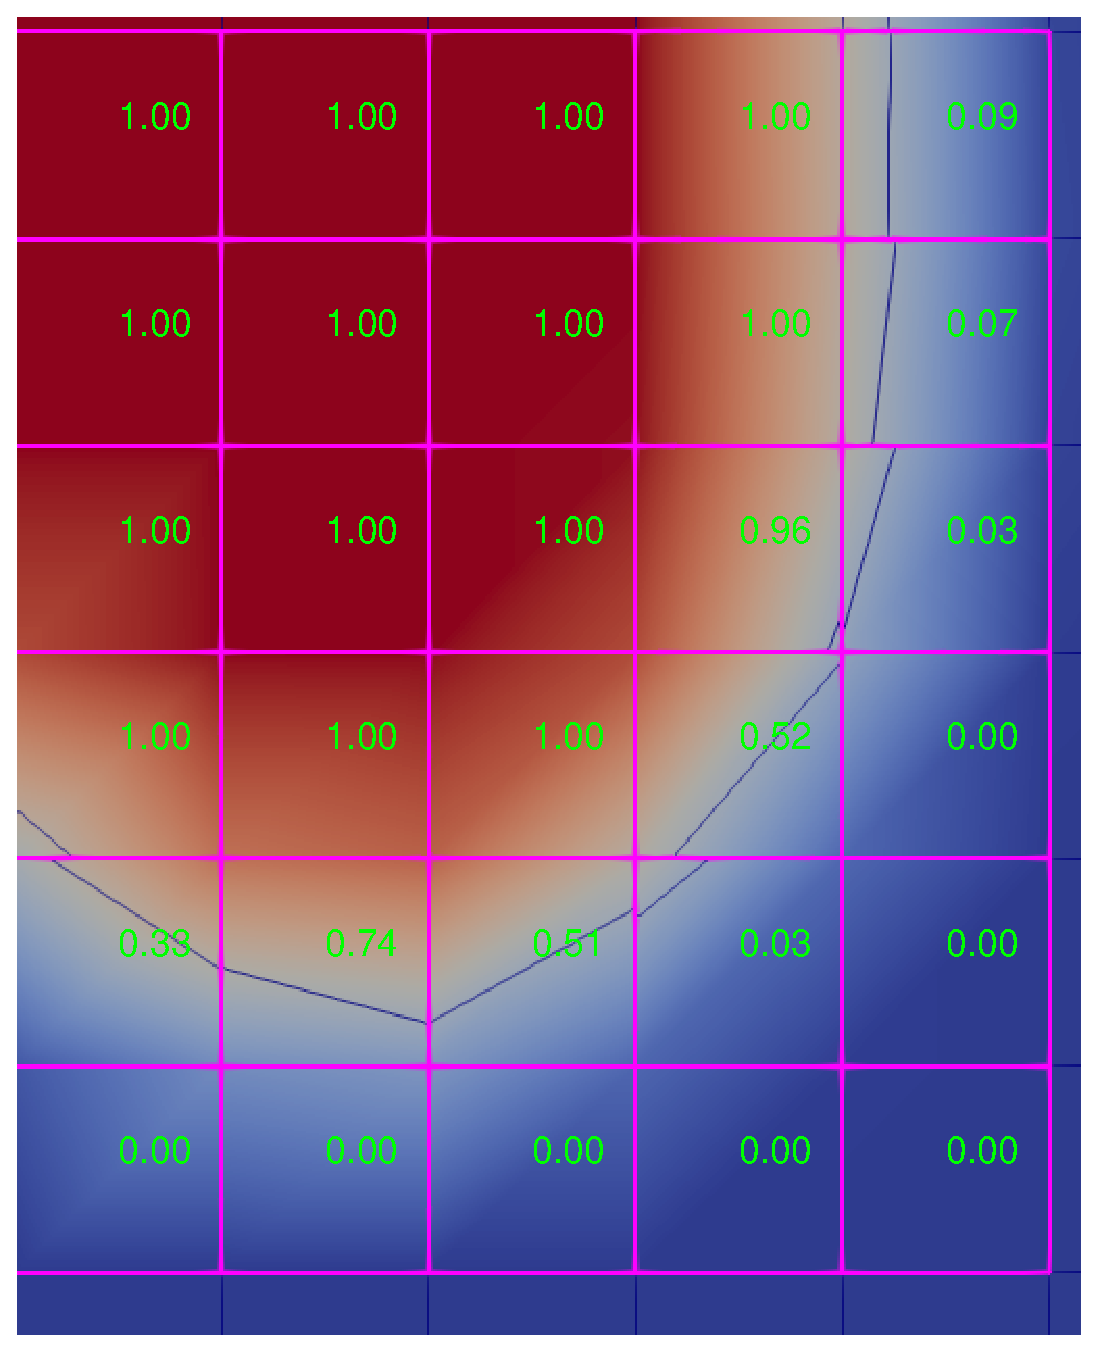
\includegraphics[width=0.4\textwidth]{noncontinuous.eps}
\caption{Noncontinuous reconstructed interfaces}
\label{fig:noncontinuous}
\end{figure}

\subsection{Interface motion}
The following equation for the volume of fluid is solved to keep the free surface conservative,
\begin{equation}\label{13}
\frac{\partial\alpha}{\partial{t}}+(\mathbf{u}\cdot\nabla)\alpha=0.
\end{equation}
As the system of all governing equations is solved in sequence within a time step, only the information about velocity field $U$, void fraction $\alpha$ and level set function $\phi$ at time $t$ is available. The void fraction field of the next time step is calculated by the following function,
\begin{equation}\label{22}
\alpha_i(t+\Delta{t})=\alpha_i(t) - \frac{1}{V_i}\sum_{j\in\mathscr{B}_i}\sigma_{ij}\int_t^{t+\Delta{t}}\int_{\mathscr{F}_i}{\Pi(\mathbf{x},\tau)\mathbf{u}(\mathbf{x},\tau)}{d\mathbf{S}d\tau},
\end{equation}
where $\sigma_ij\in{+1,-1}$, such that $\sigma_{ij}{d\mathbf{S}}$ on each cell face points from cell $i$ to cell $j$. The information between the interval $[t,t+\Delta{t}]$ is unknown. Hence it is simply estimated that the velocity field is regarded as constant during the time step. Besides, the velocity $\mathbf{u}(\mathbf{x},t)$ on the cell face is dotted with differential face normal vector, $d\mathbf{S}$, which is difficult to be integrated because of the unknown distribution of velocity on the cell face. This term can be approximated as average velocity, $u_{ij}(t)$, multiplied with differential face as follows:
\begin{equation}\label{24}
  \mathbf{u}(\mathbf{x},t)d\mathbf{S}\approx u_{ij}(t)dS =\frac{F_{ij}(t)}{S_{ij}}dS,
\end{equation}
where volumetric face flux, $F_{ij}$, is defined to estimate the average velocity on the cell faces,
\begin{equation}\label{23}
  F_{ij}(t)\equiv\int_{\mathscr{F}_{ij}}\mathbf{u}(\mathbf{x},t)d\mathbf{S}.
\end{equation}
Substitute this into (\ref{22}) and we can have
\begin{equation}\label{24}
  \alpha_i(t+\Delta{t})=\alpha_i(t) - \frac{1}{V_i}\sum_{j\in\mathscr{B}_i}\sigma_{ij}\frac{F_{ij}(t)}{S_{ij}}\int_t^{t+\Delta{t}}\int_{\mathscr{F}_i}{\Pi(\mathbf{x},\tau)dSd\tau}.
\end{equation}
The remaining face integral means the area submerged in fluid A at time t, $\mathscr{A}_{ij}(t)$,
\begin{equation}\label{25}
  \mathscr{A}_{ij}(t)\equiv\int_{\mathscr{F}_i}{\Pi(\mathbf{x},t)}dS.
\end{equation}
The volume of fluid A across each cell face in time interval $[t,t+\Delta{t}]$ can be approximated with following equation,
\begin{equation}\label{26}
  \Delta{V}_{ij}(t,\Delta{t})\approx\frac{F_{ij}(t)}{S_{ij}}\int_t^{t+\Delta{t}}\mathscr{A}_{ij}(\tau)d\tau.
\end{equation}
As above equations show, in order to calculate the void fraction $\alpha_{i}(t+\Delta{t})$ at the next time step, it is necessary to calculate the area submerged by the reconstructed interface during $\Delta{t}$ and summarize the volume of fluid A, $\Delta{V}_i$ across each face of the cell. The algorithm of estimating the interface motion was proposed by Johan Roenby \textit{et al.} and can be found in \cite{roenby2016computational}.

\subsection{Level set function initialization}
At time $t$, the void fraction field $\alpha(t)$ is known. In volume of fluid method, the normal direction $\mathbf{n}$ is calculated by following equation,
\begin{equation}\label{27}
  \mathbf{n}=\frac{\nabla{\alpha}}{\left|\nabla{\alpha}\right|}.
\end{equation}
However, $\alpha$ field has discontinuous characteristic, $\alpha\in[0,1]$, which can lead to large numerical diffusion and non-physical smearing of the interface. Hence it is difficult to obtain high precision normal direction and curvature with VOF method especially for unstructured grid \cite{cao2018coupled}. To improve the interface capturing method, level set function $\phi$ with continuous characteristic at the interface is used in CLSAdvection method. The normal direction of interface is defined as follows,
\begin{equation}\label{20}
\mathbf{n}=\frac{\nabla\phi}{\left|\nabla\phi\right|}.
\end{equation}
The level set function field $\phi(t)$ at time $t$ can be obtained from the volume fraction field $\alpha(t)$ with following steps. First, the interface cells are found with the condition that $\alpha_i\in(0,1)$ and signed with flag $0$. Secondly, find its first layer around the interface cells and sign all the first layer cell with flag $1$. Do the same with second layer cells and sign them with flag $2$. Both the layers limit the thickness of the interface and ensure its precision. Thirdly, it is assumed that the continuous interface is the iso-surface at $\alpha=0.5$ and initialize the $\phi$ with following equation,
\begin{equation}\label{28}
\tilde{\phi}(t)=1.5\varepsilon(2*\alpha(t)-1).
\end{equation}
Apparently, the first initialized level set function $\tilde{\phi}$ is not the signed distance function. There are lots of methods to re-initialize the level set function, including partial differential equation method (PDE) and fast marching method (FMM). PDE method can be easily realized in unstructured grid for it is only need to solve the following re-initialization equation, which is also a hyperbolic equation,
\begin{equation}\label{11}
\frac{\partial\phi}{\partial\tau}+sgn(\tilde{\phi})(\left|\nabla\phi\right|-1)=0,
\end{equation}
in which $sgn(\phi)$ is a sign function as following,
\begin{equation}\label{12}
sgn(x)=\left\{
\begin{array}{lc}
1,& x>0\\
0,& x=0\\
-1.& x<0
\end{array}
\right.
\end{equation}
In order to solve equation (\ref{11}), Godunov's method for discretizing the hyperbolic term  $sgn(\tilde{\phi})\left|\nabla\phi\right|$, is recommended in \cite{osher2006level}. After solving the re-initialization equation, the signed distance field $\phi$ is obtained. Nonetheless, it still need correction to ensure the mass conservative characteristic. At last, our interface can be implicitly expressed with level set function, which is confined in a band containing the interface to save computing resource. All the detailed numerical algorithms can be found in section 3.

\subsection{Normal direction and curvature}
It is already known that level set method has the advantage of computing accurate interface normal direction but the disadvantage of keeping mass conservation. Hence, the signed distance level set function $\phi$ is used to calculate the normal direction at the next time step $t+\Delta{t}$ by solving the following hyperbolic convective equation,
\begin{equation}\label{10}
\frac{\partial\phi}{\partial{t}}+(\mathbf{u}\cdot\nabla)\phi=0.
\end{equation}
Equation (\ref{10}) is sometimes referred to as the \textit{level set equation}, which was firstly proposed by Osher and Sethian \cite{osher1988fronts}. After the equation is discretized with the finite volume method (FVM), it is essential to choose a suitable scheme to compute the fluxes of $\phi$ at all boundary faces of interface cells\cite{martin2018implementation} .Because the formation of large gradients during the interface motion can cause spurious oscillations near discontinuities at the interface and lose of the interface sharpness\cite{pringuey2012large}. Using an arbitrarily Weighted Essentially Non-Oscillatory (WENO) scheme proposed by Pringuey and Cant \cite{pringuey2012high} can handle complex interface. WENO schemes have the ability to preserve the required sharpness of the interface in front-propagating problems and to deal with large gradients with discontinuities. \cite{bilger2017evaluation} takes the advantage of WENO scheme to solve equation(\ref{10}) and realize the coupled level set and volume of fluid in OpenFOAM$^{\textregistered}$ with a hyperbolic tangent function $\psi$, which is similar to Heaviside function, $H$ in equation(\ref{8}). Martin and Shevchuk\cite{martin2018implementation} apply semi-implicit WENO schemes using OpenFOAM$^{\textregistered}$ and the source code is open source used in this article's work. Besides, a third-order Total Variation Diminishing (TVD) Runge-Kutta(RK) scheme for temporal discretization is used for the advection steps\cite{pringuey2014robust}.

%\subsection{Dentisy and viscosity}
\subsection{Algorithm overview}
The numerical algorithm combines the method of volume of liquid  and level set. The solver start off with the initialization of velocity, pressure and $\alpha$ fields. Before the time loop, the LS variable, $\phi$, generate from the $\alpha$ field and create other variables like $\delta$ and $H$. Then PIMPLE loop starts from the interface reconstruction with $\alpha$ and $\vec{n}$. The figure (\ref{fig:AlgorithmProcess}) shows the specific flow chart.
\begin{figure}[htbp]
\centering
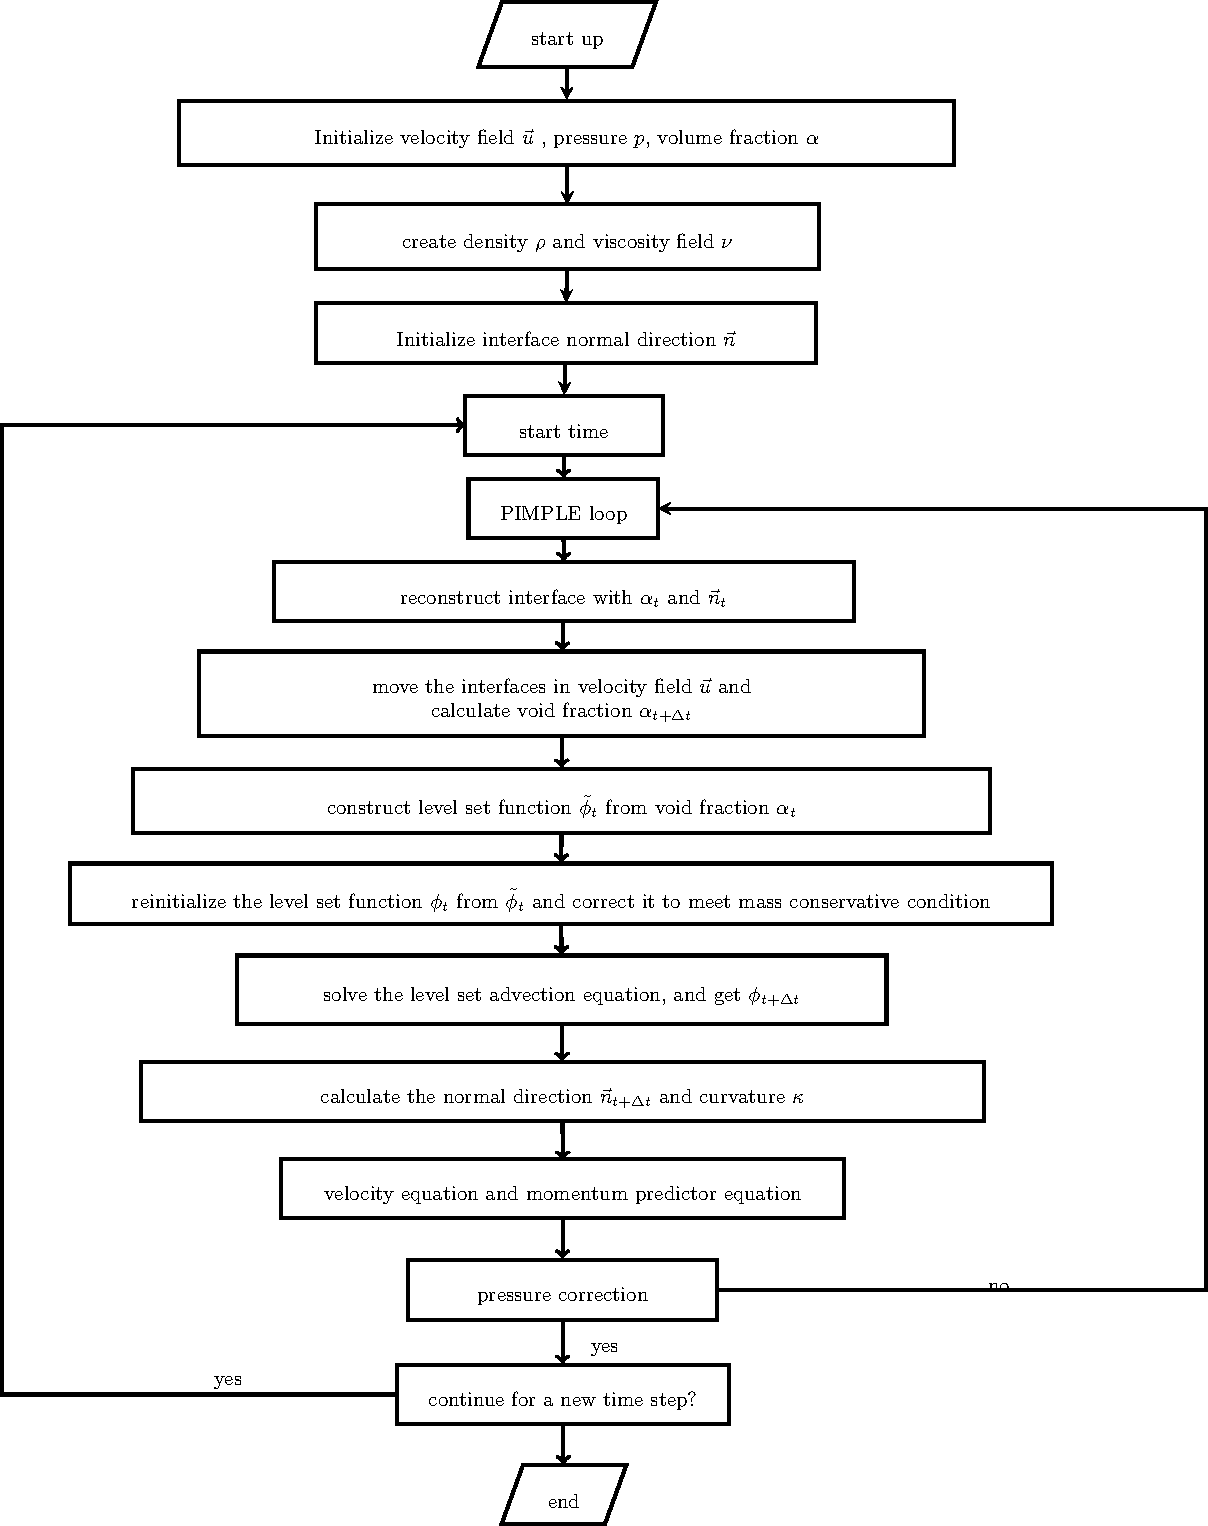
\includegraphics[width=1\textwidth]{Diagram.pdf}
\caption{Algorithm for the CLSAdvection solver.}
\label{fig:AlgorithmProcess}
\end{figure}